\chapter{Graphrepräsentationen}
\label{chap:graph_data}

Sofern im Text nicht anders vermerkt, basiert das nachfolgende Kapitel auf~\cite{linkeddatatools}.

Graphen bilden eine der Grundlagen zur Darstellung von semantischen Daten, besonders für semantische Netze. In diesem Zusammenhang spricht man auch von Graphdatenbanken.

Der Unterschied gegenüber den gängigen Datenbanken, wie zum Beispiel den relationalen oder hierarchischen Datenbanken, liegt vorallem darin, dass Objekte beliebig verknüpft werden können.

Eine Graphdatenbank ist analog einem Graphen aufgebaut. Sie nutzt also dessen Struktur, bestehend aus Knoten, Kanten und Eigenschaften, um Daten bzw. Wissen darzustellen und abzulegen. Eine Graphdatenbank ist also ein Graph mit zyklenfreier Nachbarschaft. Dies bedeudet, dass jedes Element einen direkten Verweis auf seine benachbarten Elemente enthält und somit keine Abfragen auf dessen Relationen notwendig sind.

Die Knoten einer Graphdatenbank repräsentieren Entitäten. Eigenschaften sind auf Knoten bezogene Informationen. Kanten verbinden Knoten mit Knoten oder Knoten mit Eigenschaften und stellen die Beziehung zwischen diesen dar.

\begin{figure}[htbp]
\centering \rotatebox{0}{\scalebox{0.5}[0.5]{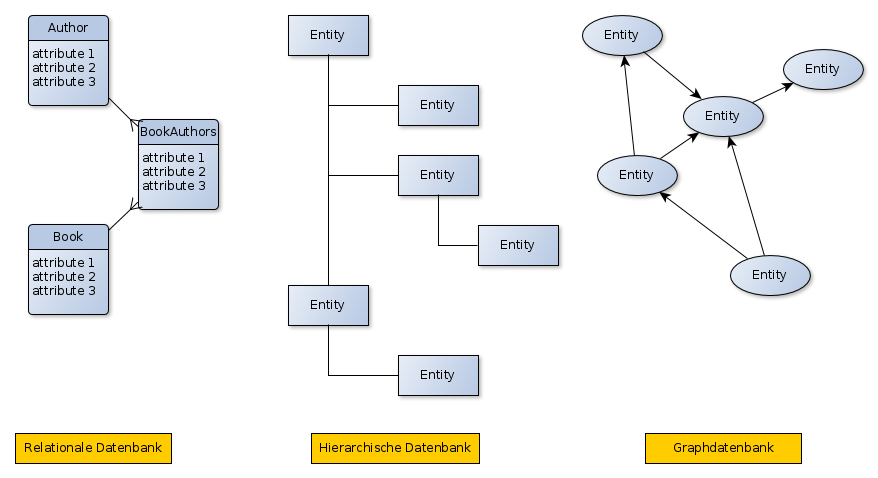
\includegraphics{bilder/datenbanktypen.png}}}
\caption{Darstellung der verschiedenen Datenbanktypen.\label{fig:datenbanktypen}\protect\footnotemark}
\end{figure}
\footnotetext{Eigene Darstellung mittels yEd, basierend auf~\cite{linkeddatatools}}

\newpage

Gegeben seien die folgenden Aussagen über Hotels:
\lstset{caption={Aussagen über Hotels\protect\footnotemark},captionpos=b}
\begin{lstlisting}
    Ein Wellnesshotel ist ein Hotel.
    Ein Familienhotel ist ein Hotel.
    Wellnesshotels sind mit Familienhotels verwandt.
\end{lstlisting}

Verwendet man diese Hotelangaben um daraus eine Graphdatenbank zu erstellen, so ergibt sich folgende Graphdatenbank:
\begin{figure}[htbp]
\centering \rotatebox{0}{\scalebox{0.5}[0.5]{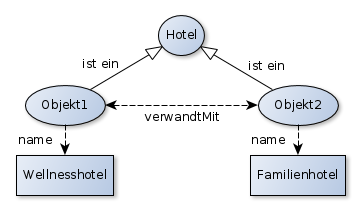
\includegraphics{bilder/hotels_graph.png}}}
\caption{Aussagen über Hotels als Graphdatenbank.\label{fig:hotels_graphdatenbank}\protect\footnotemark}
\end{figure}
\footnotetext{Eigene Darstellung mittels yEd}

In der Graphdatenbank existieren also zwei Objekte, \textit{``Objekt1''} und \textit{``Objekt2''}, mit den Eigenschaften \textit{``ist ein''}, \textit{``verwandtMit''} und \textit{``name''}.

\newpage

\noindent\rule[1ex]{\textwidth}{1pt}
\begin{wrapfigure}[6]{l}{0.1\textwidth}
    \vspace{-12pt}
    
\includegraphics[width=0.1\textwidth]{bilder/elephant.png}
\end{wrapfigure}
\label{elephant_graph_data}
Möchte man eine Graphdatenbank als Grundlage für eine semantische Datenbank aufbauen, so empfiehlt es sich, zuerst die wichtigsten Klassen und Individuen zu definieren. Es ist lohnen schon zu Beginn des Aufbaus schrittweise vorzugehen.

Nimmt man das Beispiel des Reiseplaners ist es sinnvoll, nicht von Beginn an eine komplette Reise abzubilden, sondern zunächst mit der Abbildung lokaler Ausflüge zu beginnen. Später können diese mittels Logik zu einer Reise kombiniert werden.

Nach Überlegung ergeben sich die Klassen \textit{Ausflug}, \textit{Land}, \textit{Region} und \textit{Ort}. Doch wie gelangt man zu diesen Klassen? Nach unserer Erfahrung lohnt es sich, konkrete Fragen zu stellen, welche die semantische Datenbank schliesslich beantworten können sollte. Es ist zudem hilfreich, sich praktische Beispiele von der Anwendung solch einer Datenbank zu überlegen.

So könnte eine konkrete Anwendung eine Familie sein, welche einen eintägigen Ausflug planen möchte und deren Kinder bereits in einem Alter sind, in dem sie Beschäftigung benötigen. Dies führt schliesslich zu den Kriterien \textit{familienfreundlich}, \textit{regional} und \textit{actionreich}. Dies sind ausschliesslich Überlegungen für die spätere Entwicklung des Modelles. Eine Graphdatenbank kann nicht ohne Weiteres komplexe Anfragen im Sinne der genannten Kriterien oder Inhalte beantworten. Die Zusammenhänge könnte man durch Zuweisung von Kriterien an die Objekte statisch modellieren. Dies würde jedoch den Vorteil einer semantischen Datenbank zu Nichte machen, nämlich die Gewinnung von Schlüssen aus komplexen Zusammenhängen.

Hat man Klassen und Kriterien definiert, fällt auf, dass damit noch keine konkreten Anfragen beantwortet werden können. Es fehlen die Individuen und die Relationen.\\
Daher wird für einen Ausflug das ``Individuum \textit{Seilpark Balmberg''} erstellt. Der Seilpark befindet sich in der Ortschaft \textit{Balmberg}, welche in der Region \textit{Solothurn} und damit in der \textit{Schweiz} liegt.\\
Damit erscheint es logisch, dass wenn ein Land in Regionen unterteilt ist, diese wiederum Orte beinhalten. Daher werden für Länder, Regionen und Orte ebenso Individuen erstellt.

Dies kann über die Relationen \textit{hatRegion} und \textit{hatOrt} abgebildet werden.

\begin{figure}[H]
\centering \rotatebox{0}{\scalebox{0.4}[0.4]{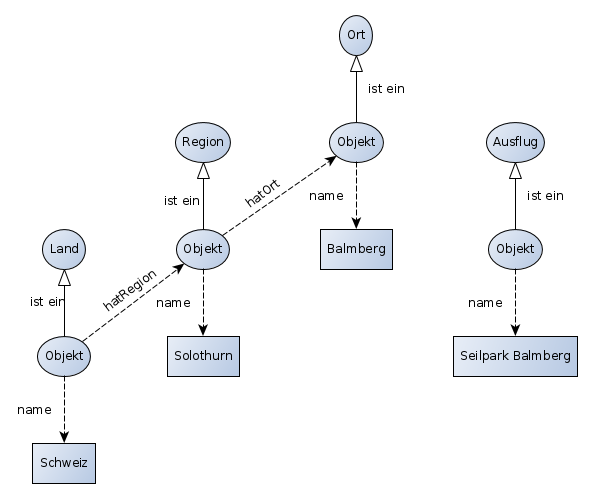
\includegraphics{bilder/graphen_beispiel_1.png}}}
\caption{Beispiel einer Graphdatenbank basierend auf dem Beispiel eines Reiseplaners\label{fig:protegebeispiel}\protect\footnotemark}
\end{figure}
\footnotetext{Eigene Darstellung mittels yEd\footnote{\url{http://www.yworks.com/en/products/yfiles/yed/}}}

Wie aus der Grafik ersichtlich, hat das Individuum \textit{Seilpark Balmberg} noch keine Relationen zu anderen Individuuen. Daher ist zum jetzigen Zeitpunkt die Verknüpfung für Mehrwert bei Abfragen unklar.

\vspace{0.1pt}
\noindent\rule[1ex]{\textwidth}{1pt}

Da eine Graphdatenbank eine hohe Abstraktionsebene darstellt, werden Wissensrepräsentationsformen sowie ihre Anwendung im folgenden Kapitel genauer erläutert.
